
% --- Auto-injected by conversion script ---
\newcommand{\currentSection}{}
\newcommand{\currentSubsection}{}

% Save original commands
\let\oldsection\section
\let\oldsubsection\subsection

% Redefine \section to update \currentSection and reset \currentSubsection
\renewcommand{\section}[1]{%
    \renewcommand{\currentSection}{#1}%
    \renewcommand{\currentSubsection}{}%
    \oldsection{#1}%
}

% Redefine \subsection to update \currentSubsection
\renewcommand{\subsection}[1]{%
    \renewcommand{\currentSubsection}{#1}%
    \oldsubsection{#1}%
}
% ------------------------------------------
\DocumentMetadata{
  lang = en-US,
  pdfversion = 2.0,
  pdfstandard = ua-2,
  tagging = on,
  tagging-setup = {math/setup=mathml-SE}
}

% Options for packages loaded elsewhere
\PassOptionsToPackage{unicode}{hyperref}
\PassOptionsToPackage{hyphens}{url}
\PassOptionsToPackage{dvipsnames,svgnames,x11names}{xcolor}
\documentclass[
  10pt,
  ignorenonframetext,
  aspectratio=1610,
]{ltx-talk}
\newif\ifbibliography
\usepackage{pgfpages}
\setbeamertemplate{caption}[numbered]
\setbeamertemplate{caption label separator}{: }
\setbeamercolor{caption name}{fg=normal text.fg}
\beamertemplatenavigationsymbolsempty
% remove section numbering
\setbeamertemplate{part page}{
  \centering
  \begin{beamercolorbox}[sep=16pt,center]{part title}
    \usebeamerfont{part title}\insertpart\par
  \end{beamercolorbox}
}
\setbeamertemplate{section page}{
  \centering
  \begin{beamercolorbox}[sep=12pt,center]{section title}
    \usebeamerfont{section title}\insertsection\par
  \end{beamercolorbox}
}
\setbeamertemplate{subsection page}{
  \centering
  \begin{beamercolorbox}[sep=8pt,center]{subsection title}
    \usebeamerfont{subsection title}\insertsubsection\par
  \end{beamercolorbox}
}
% Prevent slide breaks in the middle of a paragraph
\widowpenalties 1 10000
\raggedbottom
\AtBeginPart{
  \frame{\partpage}
}
\AtBeginSection{
  \ifbibliography
  \else
    \frame{\sectionpage}
  \fi
}
\AtBeginSubsection{
  \frame{\subsectionpage}
}
\usepackage{iftex}
\ifPDFTeX
  \usepackage[T1]{fontenc}
  \usepackage[utf8]{inputenc}
  \usepackage{textcomp} % provide euro and other symbols
\else % if luatex or xetex
  \usepackage{unicode-math} % this also loads fontspec
  \defaultfontfeatures{Scale=MatchLowercase}
  \defaultfontfeatures[\rmfamily]{Ligatures=TeX,Scale=1}
\fi
\usepackage{lmodern}
\ifPDFTeX\else
  % xetex/luatex font selection
\fi
% Use upquote if available, for straight quotes in verbatim environments
\IfFileExists{upquote.sty}{\usepackage{upquote}}{}
\IfFileExists{microtype.sty}{% use microtype if available
  \usepackage[]{microtype}
  \UseMicrotypeSet[protrusion]{basicmath} % disable protrusion for tt fonts
}{}
\makeatletter
\@ifundefined{KOMAClassName}{% if non-KOMA class
  \IfFileExists{parskip.sty}{%
    \usepackage{parskip}
  }{% else
    \setlength{\parindent}{0pt}
    \setlength{\parskip}{6pt plus 2pt minus 1pt}}
}{% if KOMA class
  \KOMAoptions{parskip=half}}
\makeatother
\usepackage{graphicx}
\makeatletter
\newsavebox\pandoc@box
\newcommand*\pandocbounded[1]{% scales image to fit in text height/width
  \sbox\pandoc@box{#1}%
  \Gscale@div\@tempa{\textheight}{\dimexpr\ht\pandoc@box+\dp\pandoc@box\relax}%
  \Gscale@div\@tempb{\linewidth}{\wd\pandoc@box}%
  \ifdim\@tempb\p@<\@tempa\p@\let\@tempa\@tempb\fi% select the smaller of both
  \ifdim\@tempa\p@<\p@\scalebox{\@tempa}{\usebox\pandoc@box}%
  \else\usebox{\pandoc@box}%
  \fi%
}
% Set default figure placement to htbp
\def\fps@figure{htbp}
\makeatother
\setlength{\emergencystretch}{3em} % prevent overfull lines
\providecommand{\tightlist}{%
  \setlength{\itemsep}{0pt}\setlength{\parskip}{0pt}}
\input{beamer-common}
\usepackage{bookmark}
\IfFileExists{xurl.sty}{\usepackage{xurl}}{} % add URL line breaks if available
\urlstyle{same}
\hypersetup{
  pdftitle={Artificial Intelligence},
  pdfauthor={Christopher Simpkins},
  colorlinks=true,
  linkcolor={Maroon},
  filecolor={Maroon},
  citecolor={Blue},
  urlcolor={blue},
  pdfcreator={LaTeX via pandoc}}

\title{Artificial Intelligence}
\author{Christopher Simpkins}
\date{}
\institute{Kennesaw State University}

\begin{document}
\frame{\titlepage}

\begin{frame}{These people are wrong.}
\protect\phantomsection\label{these-people-are-wrong.}
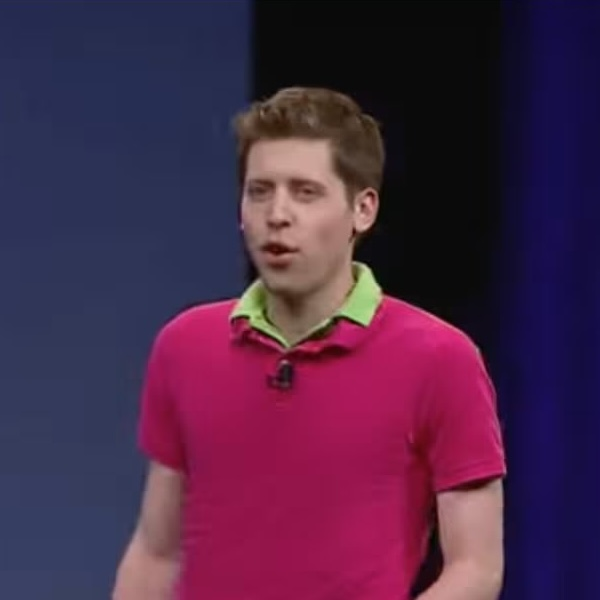
\includegraphics[width=\linewidth,height=1in,keepaspectratio]{./sam-altman-double-polo.jpg}

\includegraphics[width=\linewidth,height=1in,keepaspectratio]{./dario-amodei.jpg}
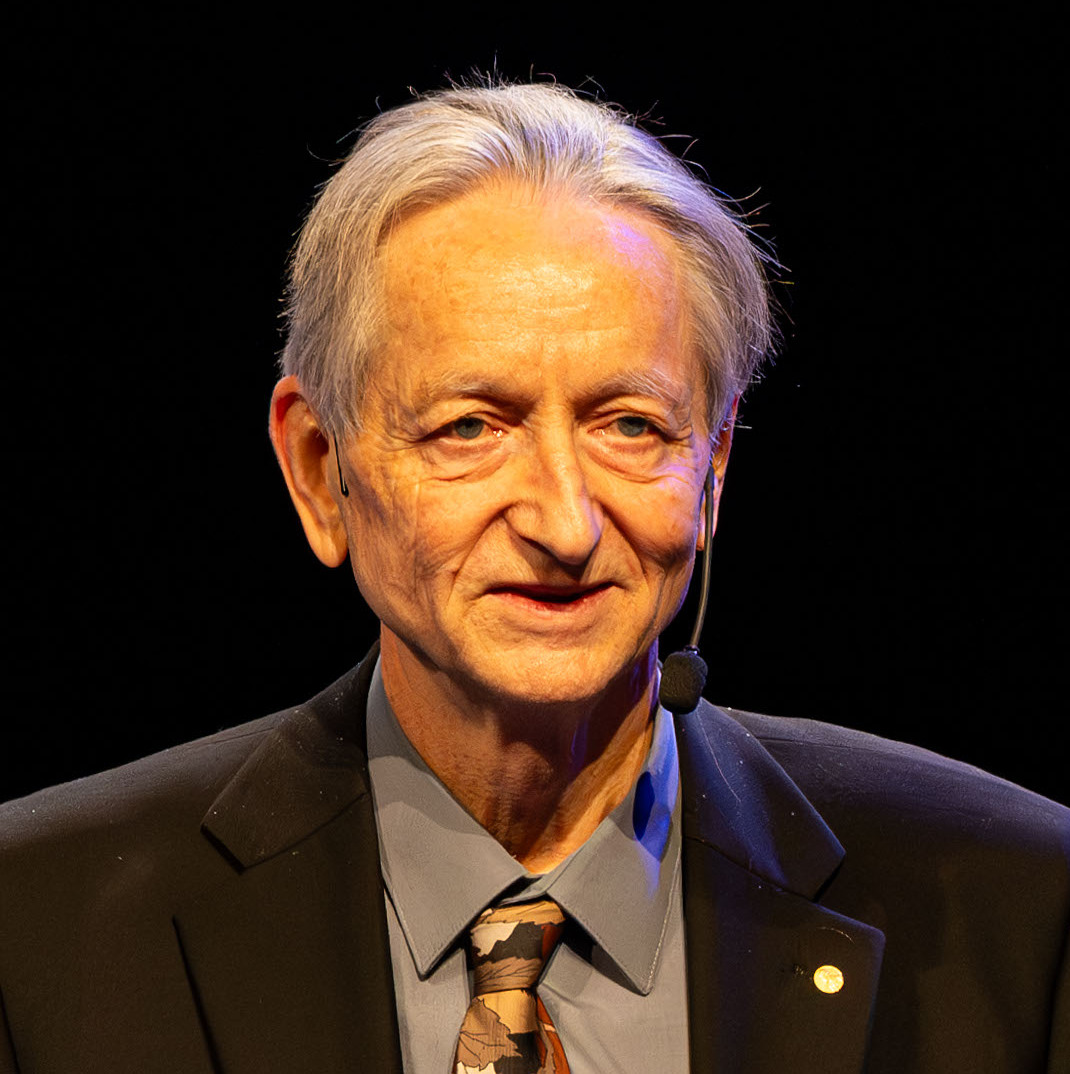
\includegraphics[width=\linewidth,height=1in,keepaspectratio]{./geoff-hinton.jpg}
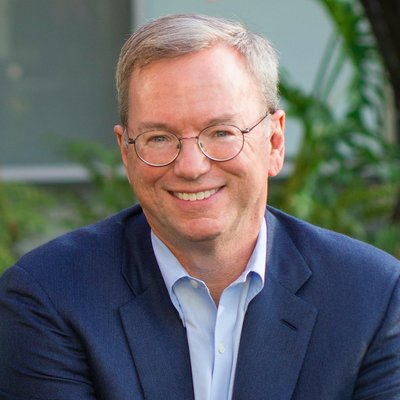
\includegraphics[width=\linewidth,height=1in,keepaspectratio]{./eric-schmidt.jpg}
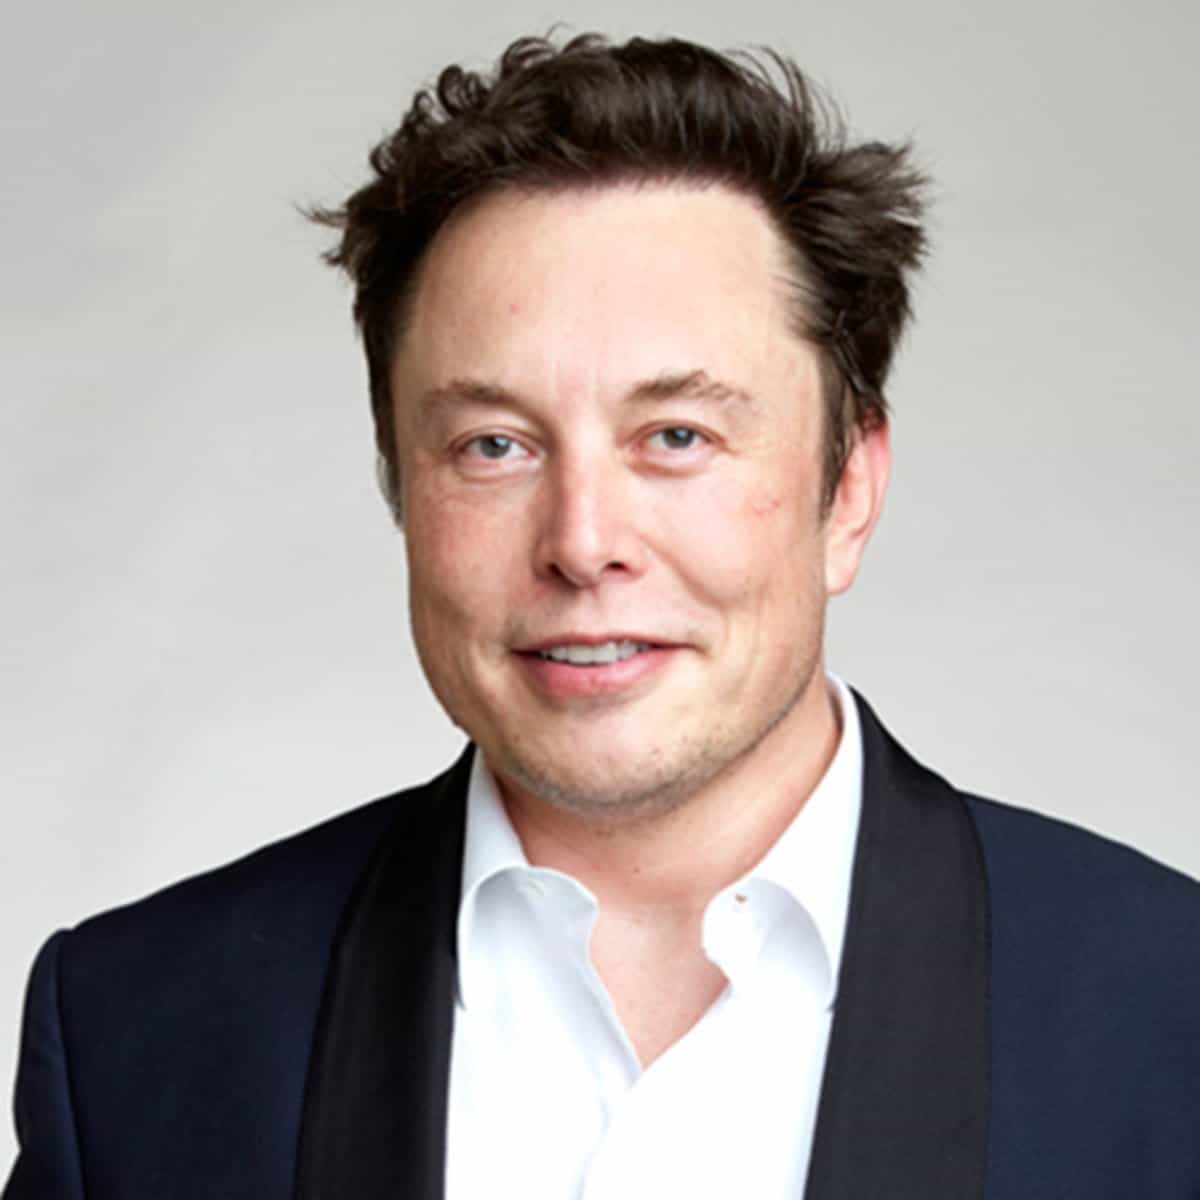
\includegraphics[width=\linewidth,height=1in,keepaspectratio]{./elon-musk.jpg}

To be fair, there are many, many people who are wrong about AI. But you
probably recognize these guys.

\begin{itemize}
\tightlist
\item
  The emergence of ``human-level AI'' has been ``just a few years away''
  since 1956. All of these predictions have been wrong.
\end{itemize}
\end{frame}

\begin{frame}{We are decades, perhaps centuries away from ``solving''
AI.}
\protect\phantomsection\label{we-are-decades-perhaps-centuries-away-from-solving-ai.}
\begin{itemize}
\tightlist
\item
  AI is immature.
\item
  Currently, unfortunately, overhyped.
\end{itemize}

\begin{center}

See my advisor's advisor's dated predictions:

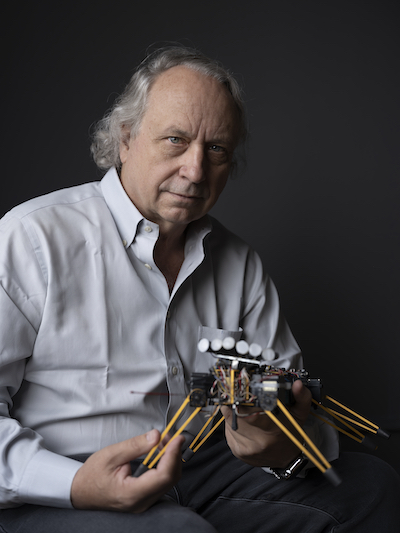
\includegraphics[width=\linewidth,height=0.3\textheight,keepaspectratio]{rodney-brooks.jpg}

https://rodneybrooks.com/my-dated-predictions/

\end{center}
\end{frame}

\begin{frame}{Why does it matter that the aforementioned hypers are
wrong?}
\protect\phantomsection\label{why-does-it-matter-that-the-aforementioned-hypers-are-wrong}
Most of the truly groundbreaking discoveries in AI are yet to be made.

\vspace{.25in}
\begin{center}
\LARGE{This makes AI exciting!}
\end{center}

\begin{itemize}
\item
  Many AI courses focus on \emph{the current thing}, e.g., statistical
  machine learning, and neural networks.
\item
  This course covers the full spectrum of AI so that you're ready to
  spot and develop promising new directions.

  \begin{itemize}
  \item
    We'll spend little time on machine learning, and barely touch on
    neural networks.

    \begin{itemize}
    \tightlist
    \item
      We have entire courses for those subjects!
    \end{itemize}
  \end{itemize}
\end{itemize}
\end{frame}

\begin{frame}{What is AI?}
\protect\phantomsection\label{what-is-ai}
\begin{columns}[T]
\begin{column}{0.5\linewidth}
\begin{center}

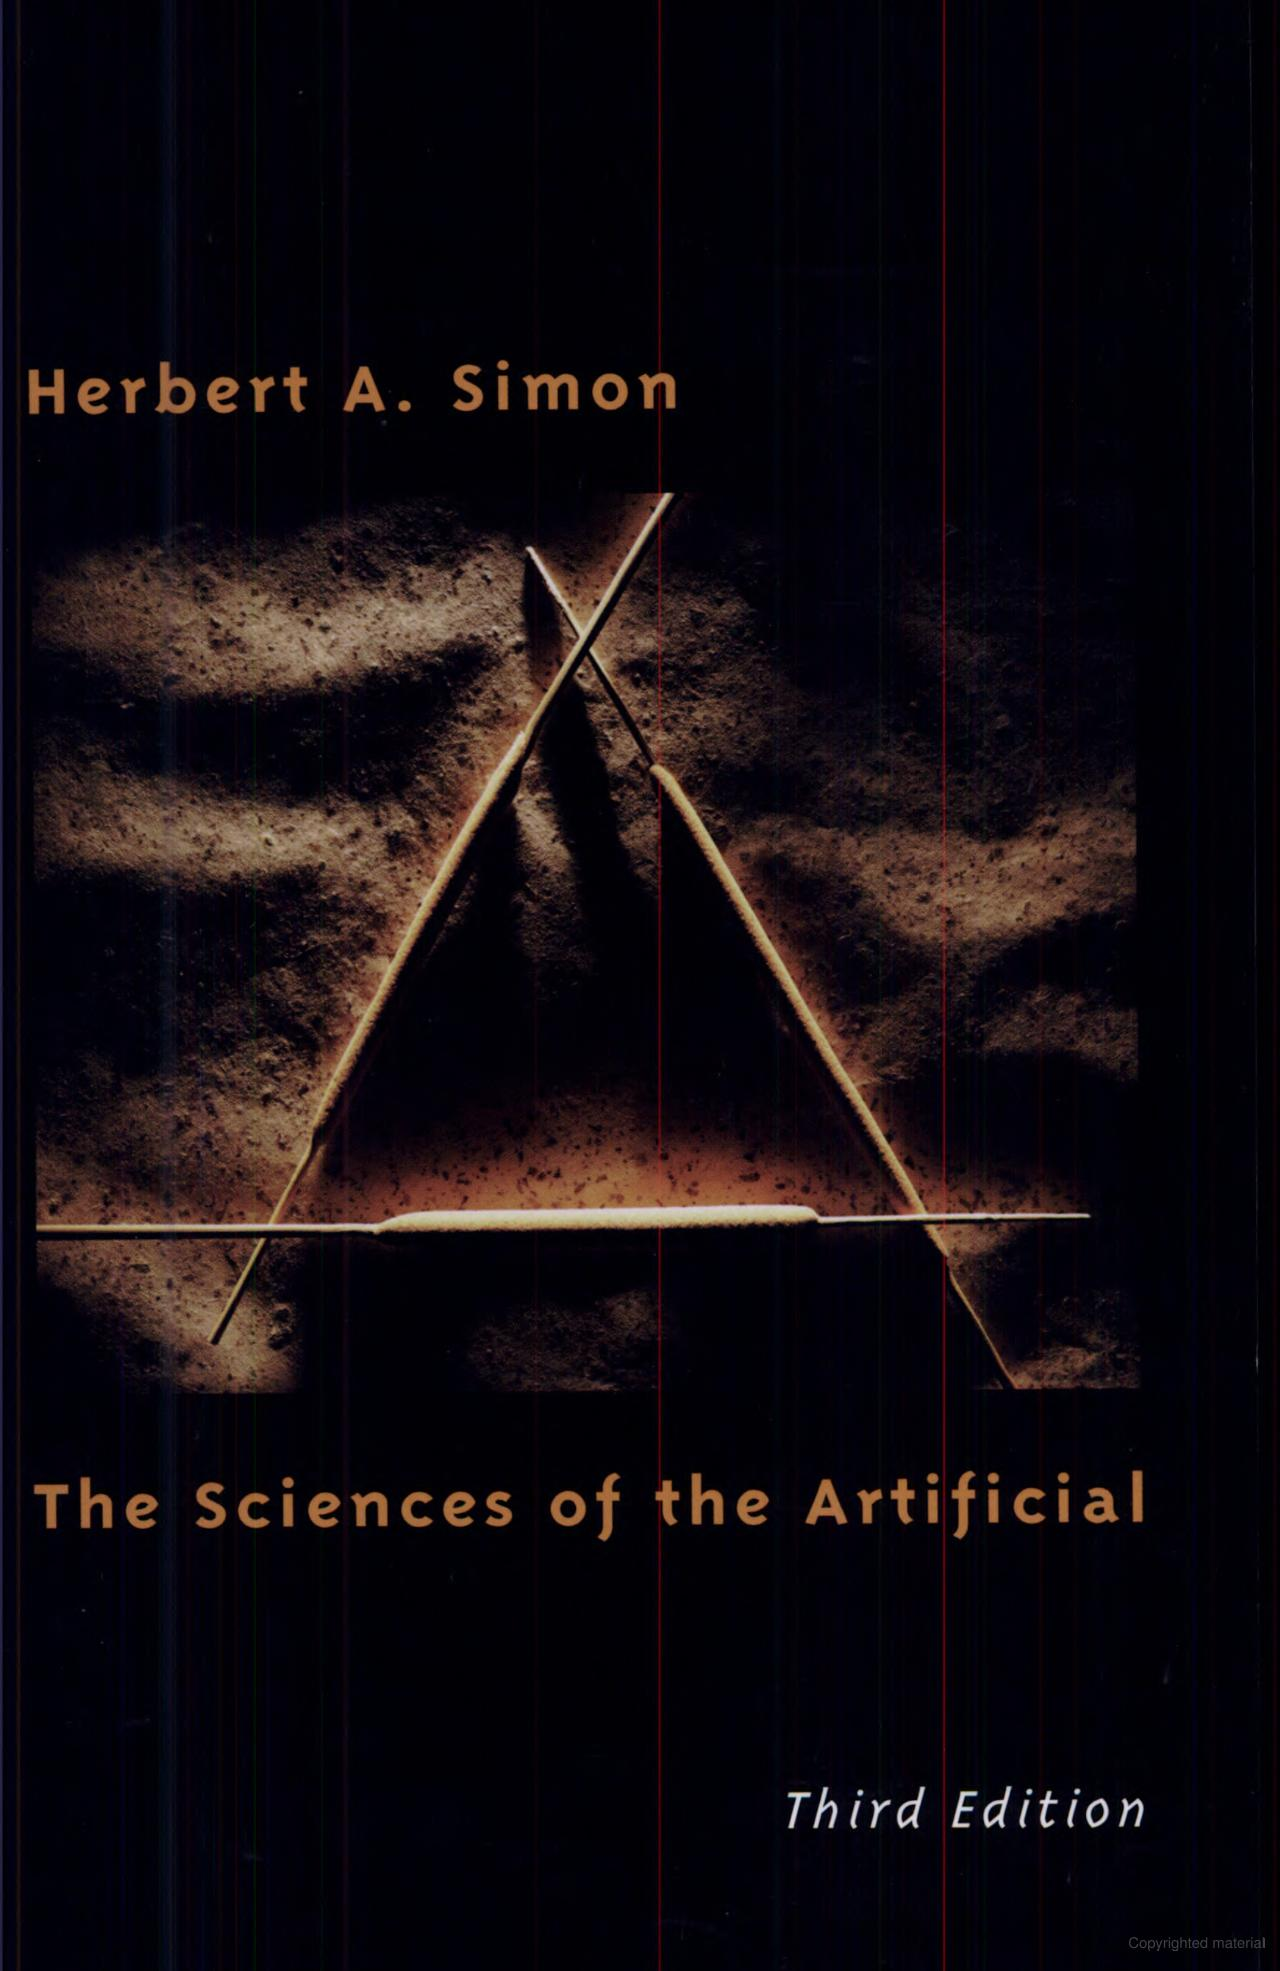
\includegraphics[width=\linewidth,height=0.6\textheight,keepaspectratio]{./simon1996sciences-cover.jpg}\footnote<.->[frame]{https://mitpress.mit.edu/9780262691918/the-sciences-of-the-artificial/}

\end{center}
\end{column}

\begin{column}{0.5\linewidth}
Artificial

\begin{itemize}
\tightlist
\item
  Man-made. Synthetic.
\end{itemize}

Intelligence

\begin{itemize}
\tightlist
\item
  Problem solving
\item
  Reasoning
\item
  Decision making
\item
  Learning
\end{itemize}

Rationality

\begin{itemize}
\tightlist
\item
  Doing the right thing.
\end{itemize}
\end{column}
\end{columns}
\end{frame}

\begin{frame}{Four Approaches to AI}
\protect\phantomsection\label{four-approaches-to-ai}
Decompose AI into thinking and acting, and define standards of
performance as fidelity to humans and quantitative rationality.

\begin{tabular}{lr|cc}\\
     &          & \multicolumn{2}{c}{Standard} \\
     &          & Humanly  & Rationally \\\hline
Mode & Acting   & Acting humanly & Acting rationally \\
     & Thinking & Thinking humanly & Thinking rationally \\
\end{tabular}
\end{frame}

\begin{frame}{Acting humanly}
\protect\phantomsection\label{acting-humanly}
Turing test

\begin{itemize}
\tightlist
\item
  Natural language processing
\item
  Knowledge representation
\item
  Automated reasoning
\item
  Machine learning
\end{itemize}

Total Turing test

\begin{itemize}
\tightlist
\item
  Computer vision
\item
  Robotics
\end{itemize}

Nobody cares about Turing tests.
\end{frame}

\begin{frame}{Rationality}
\protect\phantomsection\label{rationality}
``Doing the right thing.''

\begin{itemize}
\item
  Acting rationally - goal maximizing behavior

  \begin{itemize}
  \tightlist
  \item
    Choosing actions which reach goals with minimal cost
  \item
    Choosing actions which maximize a payoff relative to other agents
  \item
    Choosing actions which maximize long-term expected reward
  \end{itemize}
\item
  Thinking rationally - ``laws of thought''

  \begin{itemize}
  \tightlist
  \item
    Logic
  \item
    Probabilistic inference
  \end{itemize}
\end{itemize}

\begin{quote}
Thinking is nothing more than acting in an imagined space.

-- Konrad Lorenz via Bernhard Schölkopf
\end{quote}
\end{frame}

\begin{frame}{Foundations of AI}
\protect\phantomsection\label{foundations-of-ai}
\begin{itemize}
\tightlist
\item
  Philosophy
\item
  Mathematics
\item
  Neuroscience
\item
  Psychology
\item
  Computer Engineering
\item
  Control theory and cybernetics
\item
  Linguistics
\end{itemize}

Such a rich tapestry!
\end{frame}

\begin{frame}{Philosophy}
\protect\phantomsection\label{philosophy}
\begin{itemize}
\tightlist
\item
  Can formal rules be used to draw valid conclusions?
\item
  How does the mind arise from a physical brain?
\item
  Where does knowledge come from?
\item
  How does knowledge lead to action?
\end{itemize}
\end{frame}

\begin{frame}{Mathematics}
\protect\phantomsection\label{mathematics}
\begin{itemize}
\item
  What are the formal rules to draw valid conclusions?
\item
  What can be computed?
\item
  How do we reason with uncertain information?
\item
  Logic
\item
  Probability and statistics
\item
  Algorithms, computability and complexity
\item
  Optimization
\end{itemize}
\end{frame}

\begin{frame}{Economics}
\protect\phantomsection\label{economics}
Acting rationally

\begin{itemize}
\tightlist
\item
  How should we make decisions in accordance with our preferences?
\item
  How should we do this when others may not go along?
\item
  How should we do this when the payoff may be far in the future?
\end{itemize}
\end{frame}

\begin{frame}{Neuroscience}
\protect\phantomsection\label{neuroscience}
How do brains process information?

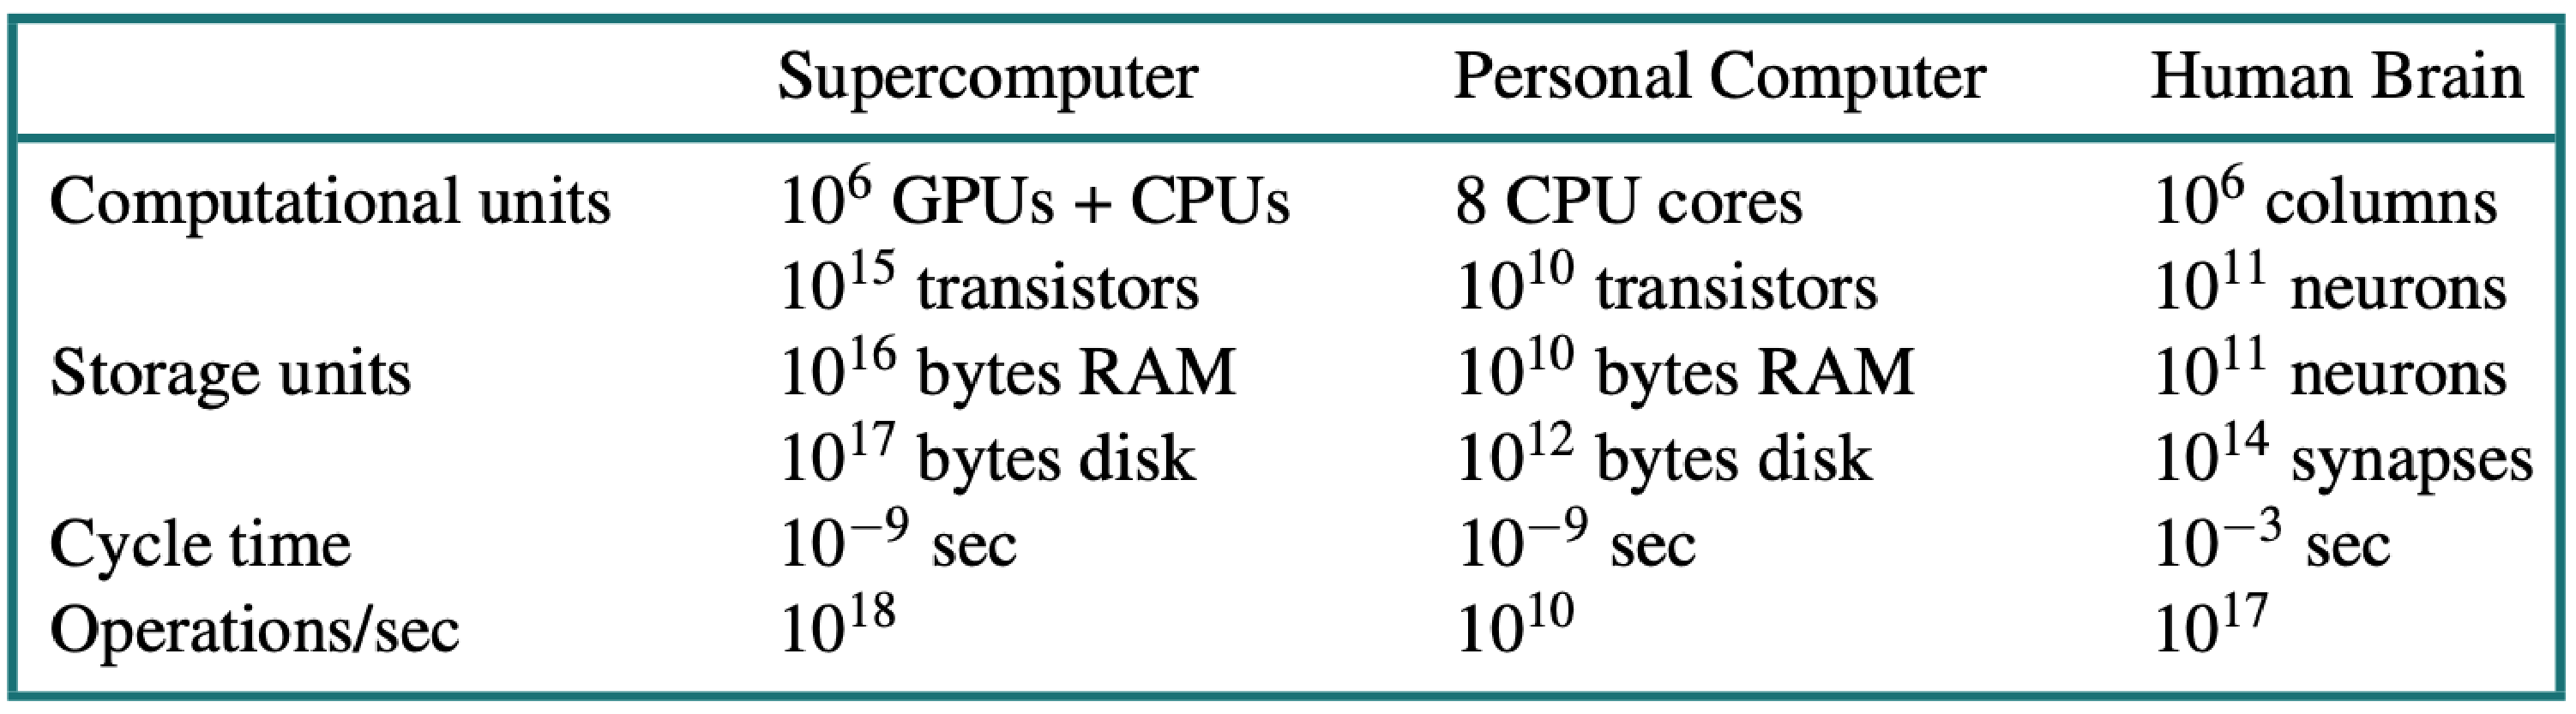
\includegraphics[width=\linewidth,height=0.5\textheight,keepaspectratio]{./aima-fig-01_02-computers-vs-brains.pdf}
\end{frame}

\begin{frame}{Psychology}
\protect\phantomsection\label{psychology}
How do humans and animals think and act?

\begin{itemize}
\item
  Cognitive modeling
\item
  Behaviorism

  \begin{itemize}
  \tightlist
  \item
    Operant conditioning
  \item
    ``Reinforcement learning''
  \end{itemize}
\end{itemize}
\end{frame}

\begin{frame}{Computer Engineering}
\protect\phantomsection\label{computer-engineering}
How can we build an efficient computer?

\begin{itemize}
\item
  High performance computing

  \begin{itemize}
  \tightlist
  \item
    Today's LLMs take years of compute time to train.
  \end{itemize}
\item
  Quantum computing
\end{itemize}

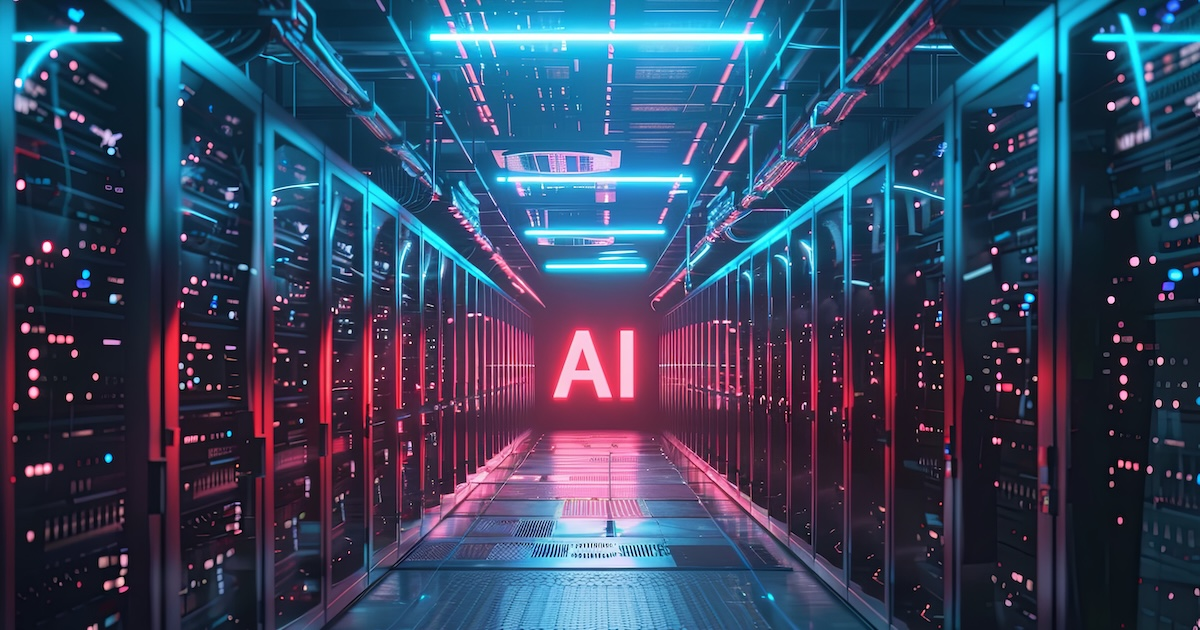
\includegraphics[width=\linewidth,height=0.5\textheight,keepaspectratio]{ai-data-center.jpg}
\end{frame}

\begin{frame}{Control theory and cybernetics}
\protect\phantomsection\label{control-theory-and-cybernetics}
How can artifacts operate under their own control?

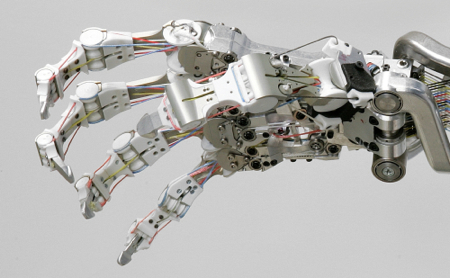
\includegraphics[width=\linewidth,height=0.3\textheight,keepaspectratio]{robot-hand.jpg}
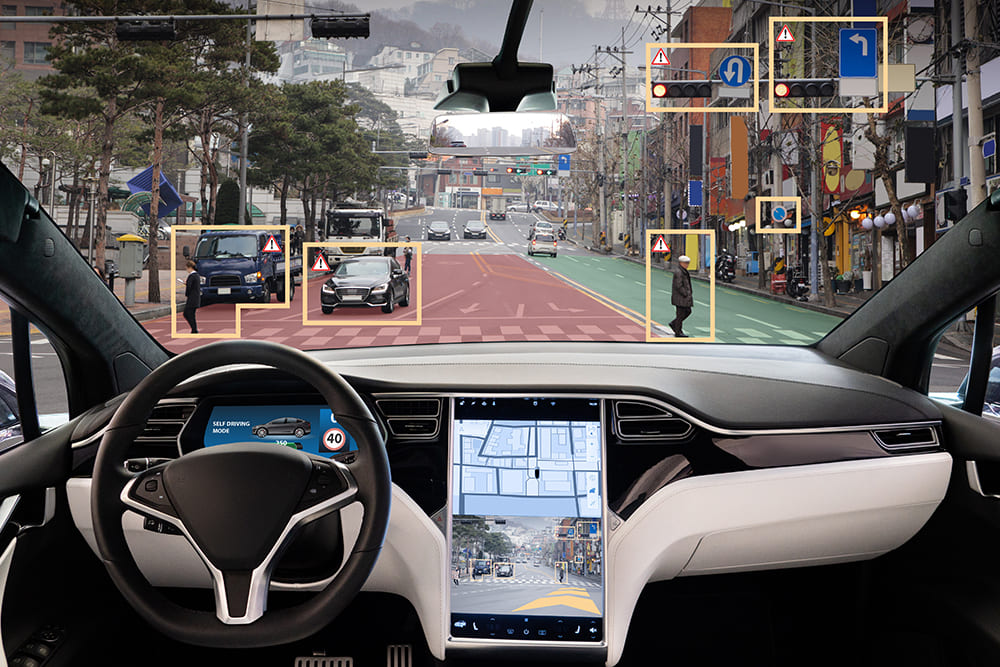
\includegraphics[width=\linewidth,height=0.3\textheight,keepaspectratio]{self-driving-car.jpg}

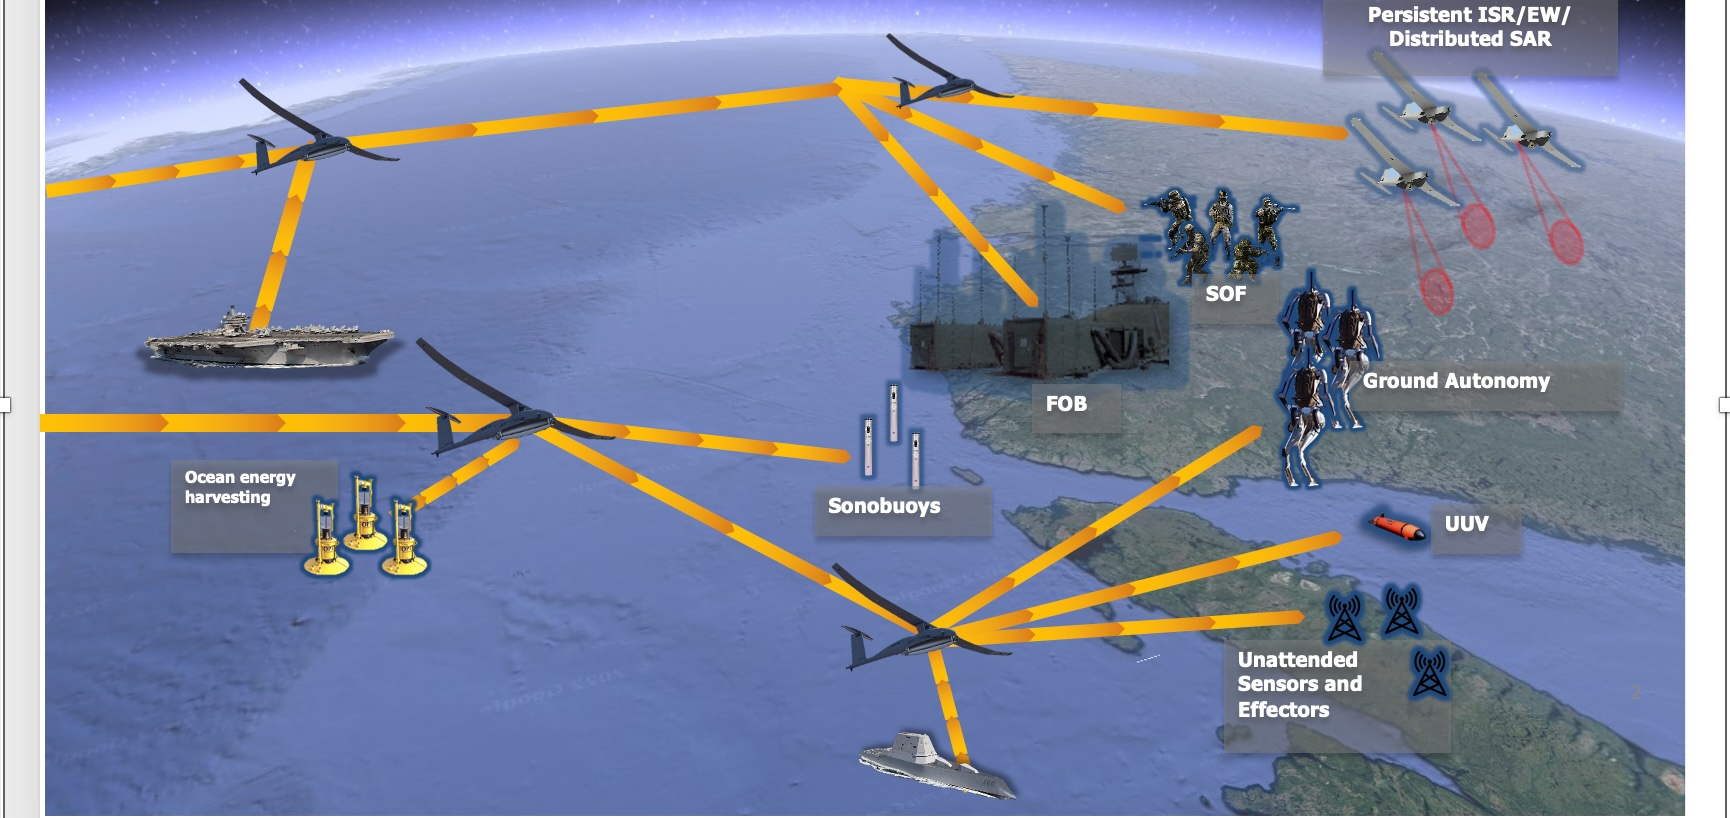
\includegraphics[width=\linewidth,height=0.3\textheight,keepaspectratio]{Power-Relay-6.jpg}

\href{https://www.darpa.mil/research/programs/power}{DARPA POWER
Program}
\end{frame}

\begin{frame}{Impact of AI}
\protect\phantomsection\label{impact-of-ai}
Turing award winners:

\begin{itemize}
\tightlist
\item
  Marvin Minsky (1969)
\item
  John McCarthy (1971)
\item
  Allen Newell and Herbert Simon (1975)
\item
  Ed Feigenbaum and Raj Reddy (1994)
\item
  Judea Pearl (1994)
\item
  Yoshua Bengio, Geoffrey Hinton, and Yann LeCun (2019)
\item
  Rich Sutton and Andrew Barto (2024)
\end{itemize}

AI lament: once an AI problem is solved, it's no longer considered AI.
\end{frame}

\begin{frame}{History of AI}
\protect\phantomsection\label{history-of-ai}
\begin{itemize}
\item
  MucCulloch, Pitts, Hebb (1943-1949)

  \begin{itemize}
  \tightlist
  \item
    Perceptrons
  \item
    Hebbian learning
  \end{itemize}
\item
  1956 Dartmouth AI Workshop

  \begin{itemize}
  \tightlist
  \item
    Organized by John McCarthy, Marvin Minsky, Claude Shannon, Nathaniel
    Rochester
  \item
    Attended by Allen Newell and Herbert Simon from Carnegie Tech,
    Trenchard More from Princeton, Arthur Samuel from IBM, and Ray
    Solomonoff and Oliver Selfridge from MIT
  \end{itemize}
\item
  Symbolic AI (1952-1969) -- ``clever Lisp programs''
\item
  First AI Winter (1966-1973)

  \begin{itemize}
  \tightlist
  \item
    Lighthill report (Lighthill, 1973) -- British government ended most
    AI funding
  \end{itemize}
\item
  Expert Systems (1969-1986)
\item
  Second AI Winter (1986)

  \begin{itemize}
  \tightlist
  \item
    Experts systems failed to deliver on their inventors' promises.
  \item
    Knowledge acquisition bottleneck.
  \item
    Adaptability, brittleness.
  \end{itemize}
\end{itemize}
\end{frame}

\begin{frame}{Modern AI}
\protect\phantomsection\label{modern-ai}
\begin{itemize}
\item
  Return of neural networks (1986-present)

  \begin{itemize}
  \tightlist
  \item
    Symbolism vs Connectionism
  \item
    Geoff Hinton, et. al.
  \end{itemize}
\item
  Probabilistic reasoning and machine learning (1987-present)

  \begin{itemize}
  \tightlist
  \item
    Neats vs scruffies
  \item
    ``Physics envy''
  \end{itemize}
\item
  Big data (2001-present)

  \begin{itemize}
  \tightlist
  \item
    Large data sets -- don't fit on a single machine
  \end{itemize}
\item
  Deep learning (2011-present)

  \begin{itemize}
  \tightlist
  \item
    You may have heard of it?
  \end{itemize}
\end{itemize}
\end{frame}

\begin{frame}{Future of AI}
\protect\phantomsection\label{future-of-ai}
\begin{columns}[T]
\begin{column}{0.3\linewidth}
\pandocbounded{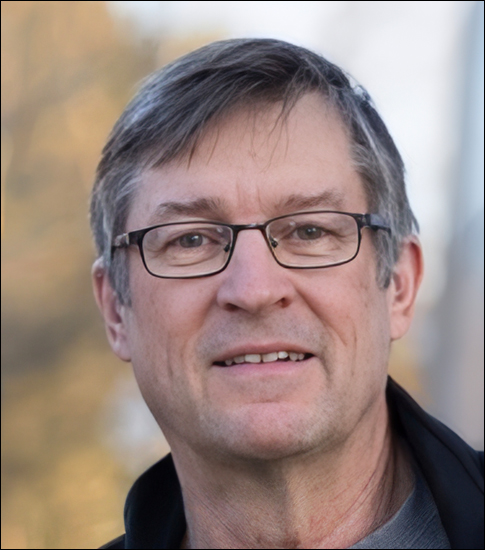
\includegraphics[keepaspectratio]{andrew-barto.jpg}}

\href{https://people.cs.umass.edu/~barto/}{Andrew Barto}
\end{column}

\begin{column}{0.3\linewidth}
\pandocbounded{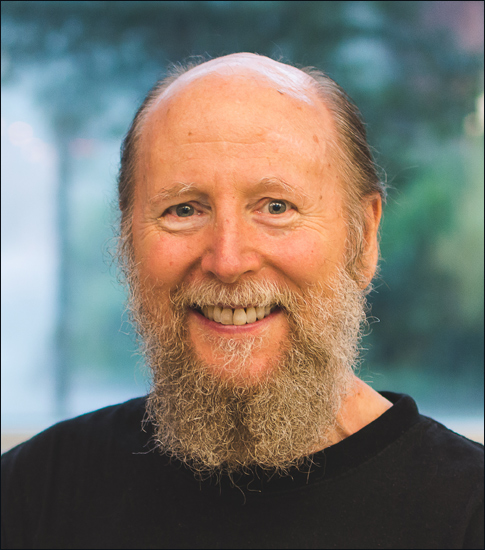
\includegraphics[keepaspectratio]{rich-sutton.jpg}}
\href{http://incompleteideas.net/}{Rich Sutton}
\end{column}

\begin{column}{0.3\linewidth}
\pandocbounded{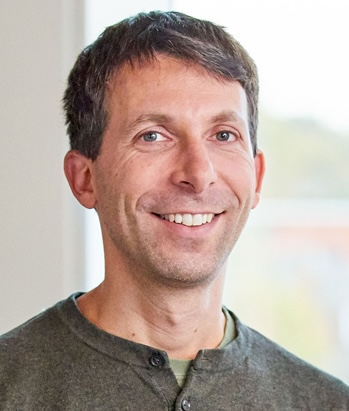
\includegraphics[keepaspectratio]{david-silver.jpg}}
\href{https://davidstarsilver.wordpress.com/}{David Silver}
\end{column}
\end{columns}

\href{https://storage.googleapis.com/deepmind-media/Era-of-Experience\%20/The\%20Era\%20of\%20Experience\%20Paper.pdf}{The
Era of Experience}
\end{frame}

\end{document}
